
\begin{appendices}
\chapter{Codes developed}




\begin{longlisting}
	\caption[Python code for generating initial list of all E3s]{Python code for generating initial list of all genes targeting E3 ligases. Requirements use Python2.7.
	\label{lst:E3list}}
	\inputminted{python}{codes/text_search2.py}
\end{longlisting}
\pagebreak
\begin{longlisting}
	\caption[Python code for getting FASTA files]{Python code for getting all FASTA files from wormbase using the gene names from the previous code as input. Requirements use Python2.7.
	\label{lst:E3fasta}}
	\inputminted{python}{codes/E3fasta.py}
\end{longlisting}


\pagebreak
\begin{longlisting}
	\caption[Jupyter notebook for visualizing RNAi screen data]{Jupyter notebook for visualizing RNAi screen data as a clustered heatmap. Requirements use Python3.8.
		\label{lst:RNAivisualize}}
	\fbox{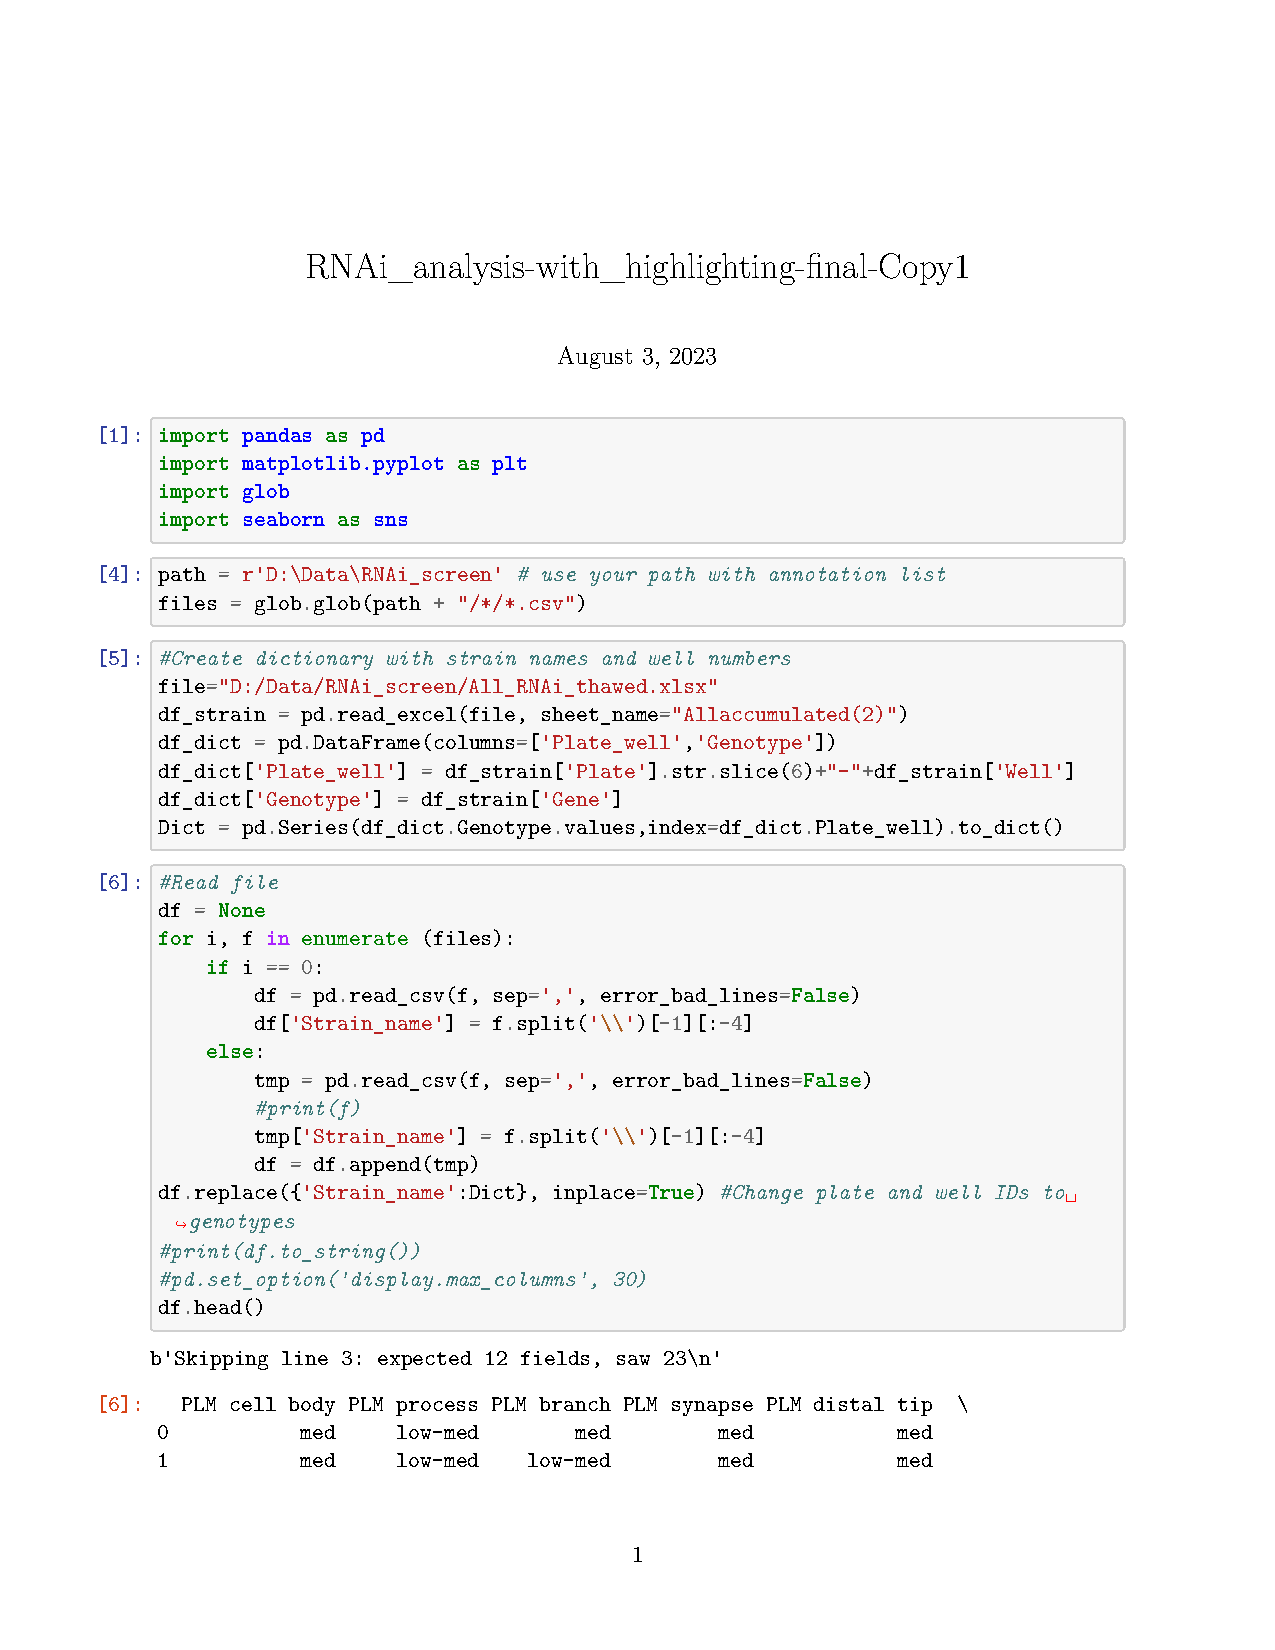
\includegraphics[page=1,scale=.78]{codes/RNAi_analysis-with_highlighting-final-Copy1.pdf}}
	\includepdf[pages=2-,frame=true,pagecommand={\pagestyle{headings}}, scale=0.8]{codes/RNAi_analysis-with_highlighting-final-Copy1.pdf}
\end{longlisting}

\end{appendices}
